%!TEX root=gm_jmlr.tex 
In this section, we define our notation and introduce some related background algorithms.
Our data consist of $n$ input vectors {$\{\x_1, \ldots, \x_n\}\! \in\! {\cal R}^p$} with corresponding labels $\{y_1, \ldots, y_n\}\!\in\!{\cal Y}$ drawn from an unknown joint distribution ${\cal D}$. Labels can be continuous (regression) or categorial (binary or multi-class classification). In this paper, we focus on feature extraction for large-scale data sets, and thus we assume that the number of inputs is much larger than the number of features ($n \gg p$). %MATT%: algorithms work for either case yeah (i.e., p >> n)? might be worth advertising both cases
%%%We also assume that each feature $\alpha$ has an acquisition cost $c_{\alpha}\! >\! 0$ during its initial retrieval. Since feature value can be cached efficiently, all subsequent retrieval on this feature is free. (maybe move into Section 4)

\subsection{The capped $l_1$-norm}
The $l_1$-norm is often used to regularize a classifier to avoid over-fitting. It is a so-called `shrinkage' operator \citep{tibshirani1996regression} in that it `shrinks' coefficients towards $0$, making the resulting solution sparse. As such, the $l_1$-norm is a popular choice in feature selection models. However, the effect of shrinkage is to reduce the magnitude of all coefficients \emph{regardless of feature quality}. To remedy this, 
%, and it also makes the solution sparse. However, these two effects are tied to each other, enforcing sparsity will also reduce the complexity of the classifier. 
\citet{zhang2009multi} introduces the \emph{capped} $l_1$-norm, which is defined by the element-wise operation:
\begin{align}
	\|\beta_j\|_{\lceil 1} = \min(|\beta_j|,\epsilon). \label{eq:cappedl1}
\end{align}
The capped $l_1$-norm is show in Figure~\ref{fig:cappedl1}. It behaves like the regular $l_1$-norm when $|\bl|$ is small, but is capped to a constant $\epsilon$ when $|\bl| \ge \epsilon$. Similar to the $l_0$-norm, the capped $l_1$-norm does not penalize large coefficients. In other words, once a feature $j$ is extracted, (i.e., $|\beta_j| > 0$) its subsequent use is not penalized as its value increases beyond $\epsilon$. When $\epsilon$ is small enough (\emph{i.e. }$\epsilon \le \min_p|\beta_j|$), the exact number of features extracted can be computed with $\frac{q_\epsilon(\bl)}{\epsilon}$. \Matt{What's $q_\epsilon$ here? I'm not exactly sure}
\begin{figure*}[t!!!]
\centerline{
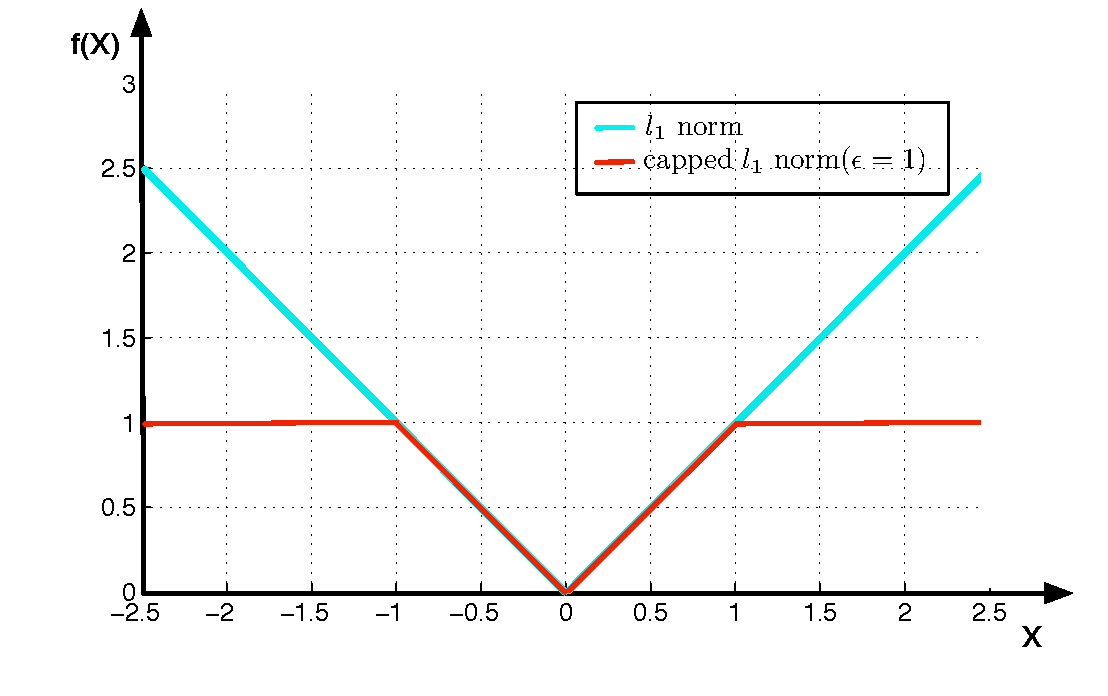
\includegraphics[width = 0.5\textwidth]{plots/cappedl1.pdf}%{plots/simul_iter}
}
\caption{The capped $l_1$-norm. It behaves like the regular $l_1$-norm when $|\bl|$ is small, but is capped to a constant $\epsilon$ when $|\bl| \ge \epsilon$.}
\label{fig:cappedl1}
\end{figure*}

\subsection{Predicting Function} We model the mapping from features to labels using a predicting function $H : {\cal R}^p \rightarrow {\cal Y}$. We learn this function by minimizing a loss function $\ell(H)$,
\begin{align}
	\min_H \ell(H). \label{eq:loss}
\end{align}
The loss function can be squared-loss for regression,
\begin{align}
	\ell_{sq}(H) = \frac{1}{n}\sum_{i=1}^n (H(\x_i) - y_i)^2, \label{eq:sqrloss}
\end{align}
or other losses such as the logistic loss for classification.

\subsection{Gradient Boosted Regression Trees (GBRT)} 
\label{sec:bg_gbrt}
Gradient Boosted Regression Trees (GBRT)~\citep{friedman2001greedy} learns the predicting function $H$ by optimizing a loss function such as (\ref{eq:sqrloss}) using gradient boosting. The learned predicting function is an additive classifier consisting of weak learners, 
\begin{align}
	H(\x) = \sum_t h_t(\x) \beta_t, \label{eq:H}
\end{align}
where $\beta_t$ is the learning rate and $h_t(\cdot)$ is a weak learner. Each weak learner $h_t \in {\cal H}$ is a regression tree \citep{breiman1984classification}, and ${\cal H}$ is the set of all possible regression trees of some limited depth $b$. At each iteration $t + 1$, a new weak learner (regression tree) is generated to minimize the loss function $\ell$. This is achieved by building a non-linear regression tree to approximate the negative gradient of $\ell$ w.r.t. current predicting function $H^t$,
\begin{align}
	h_{t+1} = \argmin_{h_{t+1}} \sum_i \Big( - \frac{\partial \ell}{\partial H^t(\x_i)} - h_{t+1}(\x_i)\Big)^2. \label{eq:CART}
\end{align}
The greedy Classification and Regression Tree (CART) algorithm \citep{breiman1984classification} is usually used to generate such a tree. Specifically, CART builds a limited depth regression tree $h_t \in {\cal H}$ by greedily minimizing an impurity function, which could be a squared loss as in (\ref{eq:CART}) for regression problems or an entropy loss for classification problems. Since in GBRT, the negative gradients $-\frac{\partial \ell}{\partial H^t(\x_i)}$ are real numbers, CART is run to minimize the squared impurity loss function (\ref{eq:CART}). It minimizes the loss function by repeatedly splitting the data on a feature per tree-node. Since CART recursively splits data using different features, it can non-linearly combine features.

From eq.(\ref{eq:H}), we see that $H$ is simply a linear function of weak learners parameterized by coefficient $\bl$, 
\begin{align}
H(\x) = \hl(\x)^\top\bl, \textrm{ where }\hl(\x) = [h_1(\x),\dots,h_T(\x)]^\top. \label{eq:boosting-trick}
\end{align}
%Each $h_t(\x) \in {\cal H}$ is a limited depth regression tree. Since ${\cal H}$ contains all possible regression trees of some limited depth, and its size $|{\cal H}| = T$ is very large, the coefficient $\bl$ is usually very sparse. This indicates that the classifier $H$ only uses a relatively small amount of trees.
%\Matt{I omitted the previous 3 sentences here} 
Imagine $h_1(\x),\dots,h_T(\x)$ is the set of all possible hypotheses in ${\cal H}$ so that $T = |{\cal H}|$. We can thus interpret the function $h(\cdot)$ as a non-linear transformation of the feature space by ${\cal H}$ as such, $\x \rightarrow \hl(\x)$, which is called the `boosting trick' \citep{friedman2001greedy,chapelle2011boosted,rosset2004boosting}. Since regression trees are negation closed (\emph{i.e.} $\forall h \in {\cal H}, \exists -h \in {\cal H}$), we assume the coefficients $\bl \ge 0$ without loss of generality. 

Finally, we define a binary indicator matrix $\Fb \in \{0,1\}^{p \times T}$. An entry in $F_{\alpha t} = 1$ if and only if feature $\alpha$ is used somewhere to split the regression tree $t$.